\chapter{Coverage} \label{cap:coverage}

\section{Test Organization and Naming}

To satisfy the requirement of separating test paradigms, the test suite was structured into dedicated packages and classes.
Line/branch tests are grouped under \texttt{sut.coverage.linebranch.*}; criterion-specific suites for
\texttt{longestPrefixOf} are in \texttt{sut.coverage.longestprefix.edgepair.\\LongestPrefixOfEdgePairTest},
\texttt{sut.coverage.longestprefix.primepath.\\LongestPrefixOfPrimePathTest}, and
\texttt{sut.coverage.longestprefix.logic.\\LongestPrefixOfConditionDecisionTest}.
Input State Partitioning for \texttt{put} is implemented in \texttt{sut.partition.put.PutBaseChoiceTest}, while
property-based testing is centralized in \texttt{sut.TSTPropertiesTest}.
All unit tests include comments describing the requirement they satisfy.

\section{Line and Branch Coverage for Public Methods}

Line and branch coverage of \texttt{TST} public methods is mainly provided by three classes. \\
\texttt{TSTCoreLineBranchCoverageTest} exercises \texttt{size}, \texttt{contains}, \texttt{get}, \texttt{put},
\texttt{keys}, \texttt{keysWithPrefix}, and \texttt{keysThatMatch}; \texttt{DeleteLineBranchTest} focuses on
\texttt{delete}; and \texttt{EqualsHashCode\\LineBranchTest} covers \texttt{equals} and \texttt{hashCode}.
The suite intentionally mixes normal behavior and guard behavior (for example, null and empty-key inputs), so both decision outcomes are observed.

\begin{figure}[H]
	\centering
	
\includegraphics[width=0.95\textwidth]{coverage/image/linebranch.png}
	\caption{Line and branch coverage evidence for public methods of \texttt{TST}}
	\label{fig:line-branch-coverage}
\end{figure}

\section{\texttt{longestPrefixOf}: Structural and Logic-Based Criteria}

Method \texttt{longestPrefixOf} was tested with three independent paradigms to avoid overfitting tests to a single test-design style.

\subsection{Edge-Pair Coverage}

In \texttt{LongestPrefixOfEdgePairTest}, tests were built around adjacent control-flow transitions.
This includes entry guards (null query and empty query), the case where the loop condition is false at the first check,
all three character-comparison outcomes (left, right, equal), and both outcomes of \texttt{x.val != null} after an equal match.

\subsection{Prime Path Coverage}

In \texttt{LongestPrefixOfPrimePathTest}, tests target maximal non-trivial paths through the loop and nested decisions.
The suite covers branch combinations such as left-then-equal and right-then-equal progressions, repeated equal transitions
with intermediate length updates, and both relevant loop-exit modes: query exhaustion and traversal falling off the trie.

\subsection{Selected Logic-Based Criterion}

Selected criterion: \textbf{Condition/Decision Coverage (CDC)}.

\textbf{Justification.}
The key control predicate in \texttt{longestPrefixOf} is:

\begin{center}
\texttt{x != null \&\& i < query.length()}
\end{center}

CDC is suitable compared to stronger alternatives like RACC or CACC because it focuses on the critical decision without requiring all combinations of conditions. In this case, RACC or CACC would require at most 4 test cases beyond what CDC already demands with marginal gains.
CDC is more appropriate than weaker criteria like C0 or D0 because it ensures that both the true and false outcomes of the decision are tested, which is essential for validating the method's behavior under different input scenarios.
Accordingly, \texttt{LongestPrefixOfConditionDecision\\Test} includes scenarios where the predicate is true, false due to
\texttt{x == null}, and false due to \texttt{i < query.length()} becoming false, plus tests for nested character-comparison branches.

\begin{figure}[H]
	\centering
	
\includegraphics[width=0.95\textwidth]{coverage/image/longestprefix.png}
	\caption{Coverage-oriented test evidence for \texttt{longestPrefixOf} (edge-pair, prime-path, and CDC suites)}
	\label{fig:longestprefix-coverage}
\end{figure}

\section{ISP Base Choice Coverage for \texttt{put}}

\texttt{PutBaseChoiceTest} implements Base Choice Coverage from the required partitions.
The base configuration is an empty trie with a typical new key; each variation changes one characteristic at a time,
including an existing identical key, an existing prefix of the new key, and lexicographic position (smallest, largest,
typical) in a non-empty trie.
An explicit null-key guard test is included as input validation support.

\begin{figure}[H]
	\centering
	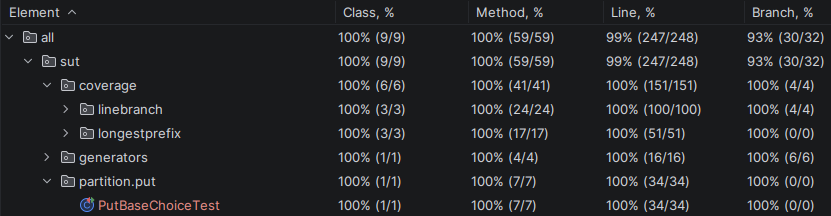
\includegraphics[width=0.90\textwidth]{coverage/image/partition.png}
	\caption{Input State Partitioning and Base Choice tests for \texttt{put}}
	\label{fig:put-partition-coverage}
\end{figure}

\section{Property-Based Testing with JUnit QuickCheck}

Property tests are implemented in \texttt{TSTPropertiesTest} using a custom generator
\texttt{sut.\\generators.TSTGenerator}.
The generator produces random tries with a mix of independent keys and related-prefix keys, which is useful for stressing trie-specific behavior.

The implemented properties verify that insertion order of distinct keys does not alter the final trie value, deleting all keys leaves the trie empty, inserting and then removing the same fresh key restores the initial tree, and a stricter prefix in \texttt{keysWithPrefix} yields a strict subset whenever the generated trie distinguishes both prefixes.
These checks depend on semantic equality and therefore rely on the implemented \texttt{equals()} method in the SUT.

\section{Reproducibility Commands}

The following commands can be included in the report to reproduce test execution.

\begin{verbatim}
# Run full test suite
mvn clean test

# Run only line/branch package
mvn -Dtest=sut.coverage.linebranch.* test

# Run only longestPrefixOf criterion classes
mvn -Dtest=sut.coverage.longestprefix.edgepair.LongestPrefixOfEdgePairTest test
mvn -Dtest=sut.coverage.longestprefix.primepath.LongestPrefixOfPrimePathTest test
mvn -Dtest=sut.coverage.longestprefix.logic.LongestPrefixOfConditionDecisionTest test

# Run put() ISP Base Choice suite
mvn -Dtest=sut.partition.put.PutBaseChoiceTest test

# Run QuickCheck properties
mvn -Dtest=sut.TSTPropertiesTest test
\end{verbatim}